\subsection{Evolução da atitude e modos de operação}
\label{sec_cap4_app_final_atitude}

Ao longo da simulação, a atitude do perseguidor permanece estabilizada em torno da orientação de referência do alvo por conta da lei de controle implementada do tipo \gls{pd}.
As variações mais pronunciadas observadas nos ângulos de Euler $\phi$ (X,roll), $\theta$ (Y, pitch) e $\psi$ (Z, yaw) concentram-se em transientes rápidos logo após a entrada do controlador de atitude, com duração de alguns segundos, e são associados à aplicação instantânea do comando de controle.
Esses transientes são interpretados como ruído de curta duração e não alteram o resultado final da manobra.
Ao final da aproximação, os erros de atitude convergem para valores próximos de zero, caracterizando um alinhamento consistente do perseguidor em relação ao referencial do alvo e que está dentro do limite máximo estabelecido de $\pm 1^{\circ}$.
A Tabela~\ref{tab_cap4_app_curta_erros_atitude} apresenta os erros de atitude medidos no início da aproximação de curta distância até o final da missão, ambos em relação ao alvo.

\begin{table}[H]
\centering
\caption{Erros de atitude inicial e final do perseguidor em relação ao alvo.}
\label{tab_cap4_app_curta_erros_atitude}
\begin{tabularx}{\linewidth}{|
  >{\centering\arraybackslash}X|
  >{\centering\arraybackslash}X|
  >{\centering\arraybackslash}X|}
\hline
\textbf{Ângulo} &
\textbf{Erro inicial [grau]} &
\textbf{Erro final [grau]} \\
\hhline{|=|=|=|}
$x$ (roll)   & $7{,}0^\circ$  & $0{,}098^\circ$ \\
$y$ (pitch)& $8{,}0^\circ$  & $0{,}023^\circ$ \\
$z$ (yaw)    & $9{,}0^\circ$  & $0{,}299^\circ$ \\
\hline
\end{tabularx}
\end{table}

A Figura~\ref{fig_cap4_atitude_grau} apresenta a evolução da atitude do perseguidor ao longo da aproximação, evidenciando seu alinhamento em relação à atitude da espaçonave alvo.
O primeiro subgráfico mostra a resposta completa em ângulos de Euler, do início da aproximação curta até momentos posteriores ao acoplamento.
Por sua vez, o segundo subgráfico corresponde a um recorte temporal a partir de $400$ s até o término da simulação, com o objetivo de destacar o comportamento da atitude após a habilitação do manipulador robótico e, portanto, durante a fase em que a dinâmica acoplada espaçonave--manipulador passa a atuar.

Por fim, o terceiro subgráfico apresenta um destacamento maior do intervalo inicial, para visualizar com maior detalhe o transiente associado às condições iniciais e à entrada em operação simultânea das malhas e modelos do sistema (controle de atitude, dinâmica do corpo rígido e movimento translacional relativo descrito pelas equações de \gls{hcw}).

\begin{figure}[H]
\centering
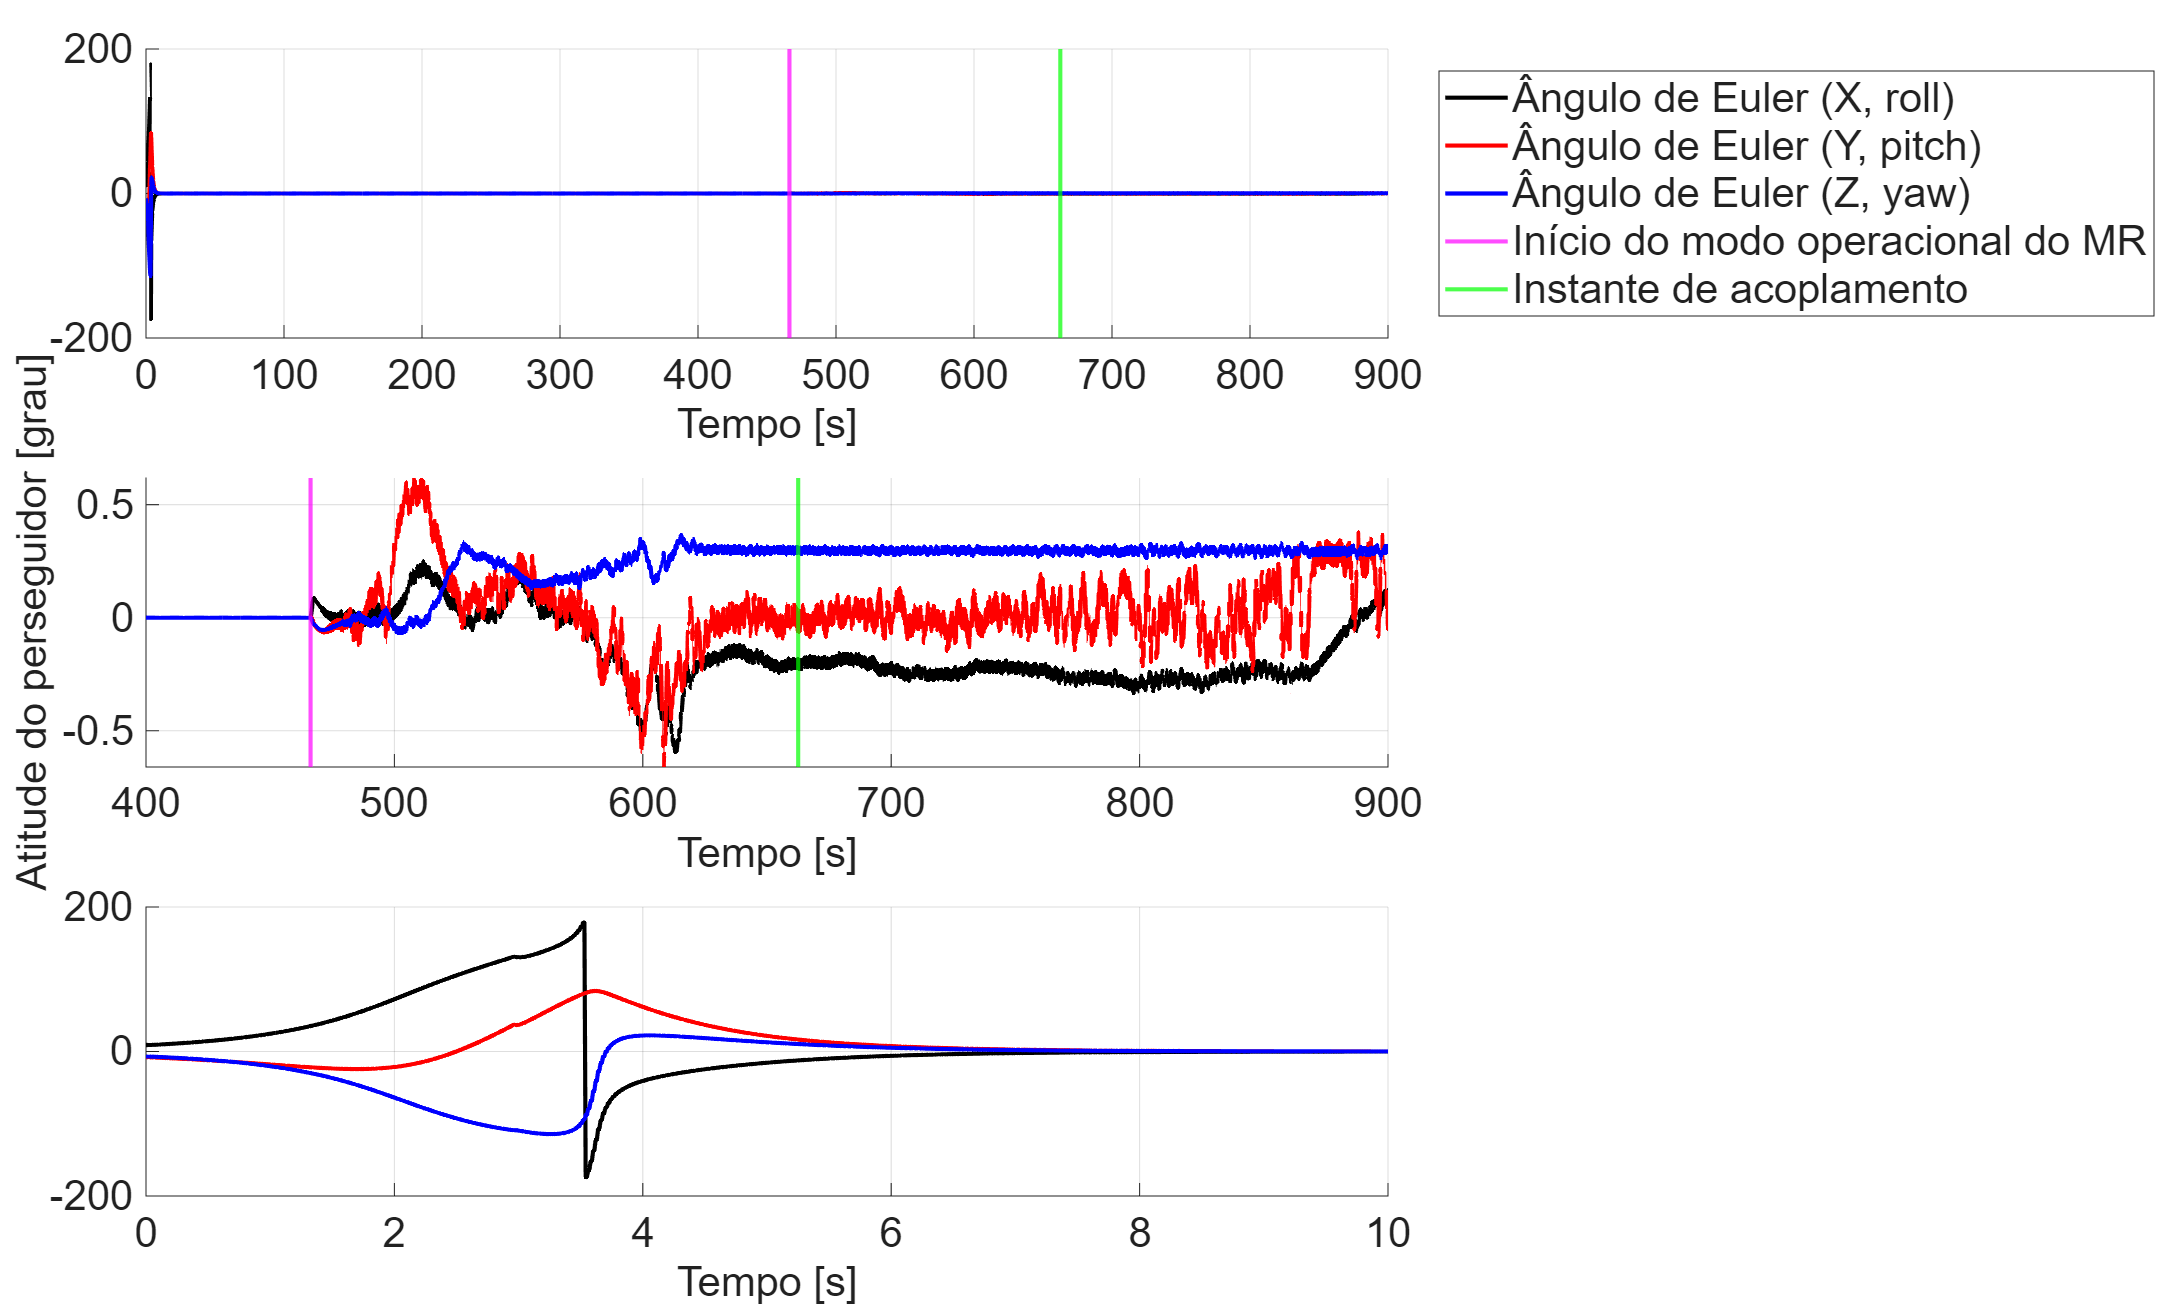
\includegraphics[width=1\linewidth]{5 Resultados/Imagens/3 App final/1A Atitude perseguidor.png}
\caption{Atitude do perseguidor em ângulos de Euler ao longo de toda a aproximação.}
\label{fig_cap4_atitude_grau}
\end{figure}

A linha vertical rosa em $t = 466{,}26$ s indica o instante de habilitação do \gls{mr}.
A linha vertical verde indica o instante de acoplamento entre as espaçonaves.
O modo de operação do modelo inicialmente corresponde à fase sem atuação do manipulador, e transita para o modo de operação do \gls{mr}, mantendo-se desta forma até o final da simulação.

Assim, a aproximação final ocorre integralmente com o manipulador ativo, enquanto que o controle de atitude do corpo compensa os efeitos de reação da espaçonave decorrentes do movimento das juntas, preservando o alinhamento de atitude do perseguidor ao longo da manobra.
Em paralelo, o controle translacional relativo permanece ativo durante todo o trecho final, sendo a dinâmica relativa propagada pelas equações de \gls{hcw} e pela respectiva lei de controle definida para a aproximação em \gls{lvlh}.
